\subsection{Zarys metody}
Ta część projektu polegała na zaimplementowaniu metody detekcji steganografii opisanej w pracy \cite{dct_match_article}, działającej na obrazach. Metoda opiera się na wyznaczeniu cech obrazu służących jako dane wejściowe klasyfikatora. Cechy są wyznaczane poprzez porównywanie wzorców występujących we współczynnikach DCT obrazu przed i po operacji croppingu. Okazuje się że obrazy poddane steganografii (stego-images) mają inny rozkład cech niż oryginalne obrazy (cover-images), co pozwala na skuteczną klasyfikację.\\

\subsection{Wykorzystane Dane}
Metoda ta w ogólności znajduje zastosowanie w tak zwanej Blind-Steganalysis, czyli próbie detekcji steganografii przy braku wiedzy o metodzie wykorzystywanej do ukrycia wiadomości. W mojej implementacji skupiłem się na detekcji wiadomości ukrytych za pomocą prostego LSB-substitution, w obrazach o wymiarach 256x256 pikseli, w odcieniu szarości. W tym celu zaimplementowałem algorytm przeporwadzający LSB-substitution dla obrazów (.png), a następnie dla zbióru obrazów o podanych wymiarach, wygenerowałem ich wersje stego, gdzie ukrywałem wiadomości, o długości odpowiadającej użyciu około 15\% dostępnego nośnika.\\ 

\subsection{Opis metody}
Ogólny schemat działania algorytmu prezentuje diagram \ref{fig:dct_match_scheme}.
\begin{figure}[ht!]
	\centering
	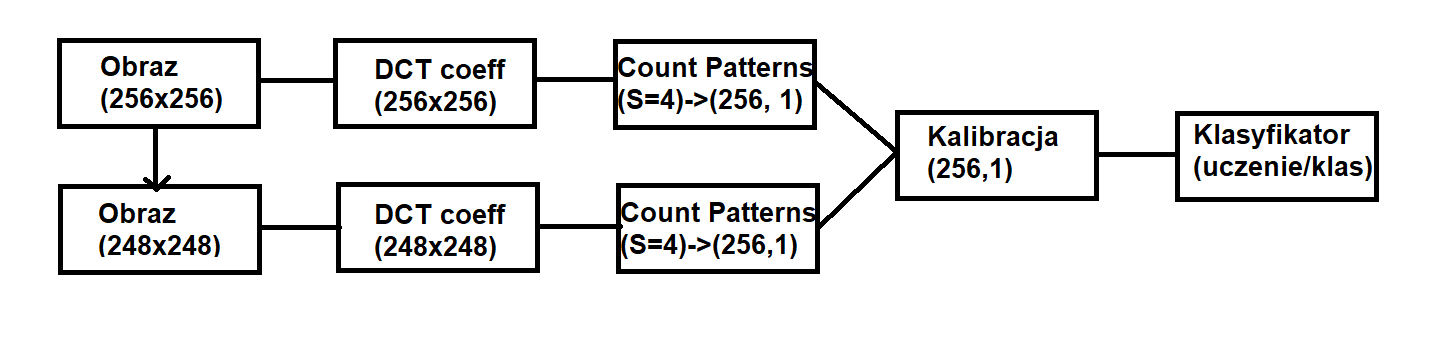
\includegraphics[width=0.8\textwidth]{./img/dct_match_scheme.png}
	\caption{\label{fig:dct_match_scheme} Schemat uczenia/klasyfikacji.}
\end{figure}

W fazie uczenia obrazy wczytywane są wraz z odpowiadającymi im klasami (stego albo cover). Następnie wyznaczane są współczynniki DCT oraz zliczane są ilości występujących w nich wzorców. Te same operacje powtarzane są dla "okrojonej" (cropped) wersji obrazu. Poprzez kalibrację, polegającej na porównaniu ilości wzorców w oryginalnym obrazie i jego okrojonej wersjii wyznaczany jest wektor cech, który przekazywany jest do klasyfikatora. W fazie uczenia, do klasyfikatora przekazywana jest również klasa obrazu, a parametry klasyfikatora są aktualizowane na podstawie danych. W fazie klasyfikacji, wektor cech bez klasy przekazywany jest do nauczonego już klasyfikatora w celu wykonania predykcji klasy.\\

Okrojenie obrazu (Image Cropping), polega na stworzeniu nowego obrazu będącego wycinkiem poprzedniego. W zaimplementowanej metodzie, obraz "obcina" się o 4 piksele wzdłuż każdej krawędzi, otrzymując tym samym nowy obraz o wymiarach:
\begin{equation}
    (H_{crop}, W_{crop}) = (H - 8, W - 8)
\end{equation}
gdzie $H$ i $W$ to wymiary oryginalnego obrazu.\\

Następnie, dla obu obrazów wyznacza się ich współczynniki DCT. Z otrzymanych macierzy współczynników, dla obu obrazów zlicza się wzorce zdefiniowane przez następujący algorytm opisany w pracy \cite{dct_match_article}. Dany jest parametr $S$ algorytmu. Różnica między dwoma współczynnikami $x$, $y$ zdefiniowana jest jako:
\begin{equation}
    d(x, y) = Max(|x-y|,\space S-1)
\end{equation}
co zapewnia ograniczenie górne odległości. Zgodnie z oryginalną pracą, w implementacjii zastosowano wartość parametru $S=4$. Po całej macierzy współczynników obrazu iteruje się ramką w postaci pokazanej na rysunku \ref{fig:pattern_window}.
\begin{figure}[ht!]
	\centering
	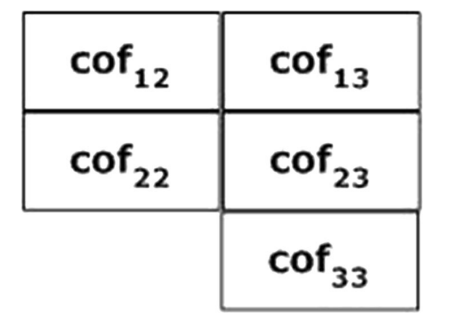
\includegraphics[width=0.5\textwidth]{./img/dct_match_pattern_window.png}
	\caption{\label{fig:pattern_window} Ramka schematów. Źródło:DOI: 10.1007/s11042-017-4676-z}
\end{figure}

Dla danej pozycji ramki wyznacza się dwie wartości referencyjne (minimalną oraz maksymalną wartość współczynnika w ramce). Następnie dla każdej wartości referencyjnej oblicza się odległości między wartością referencyjną a pozostałymi wartościami w ramce, oraz tworzy się wzór $P$ będący 4-elementowym wektorem postaci:
\begin{equation}
    P = (d(l, b),\space d(ul,b), \space d(ur, b), \space d(r, b))
\end{equation}
gdzie $b$ oznacza wartość referencyjną, a $l, ul, ur, r$ to wartości pozostałych współczynników ramki. Kolejność tych współczynników zależy od tego, na jakiej pozycji znajdował się współczynnik referencyjny. Wpływ pozycji współczynnika referencyjnego na kolejność współrzędnych wektora $P$ pokazuje rysunek \ref{fig:coeff_order}.
\begin{figure}[ht!]
	\centering
	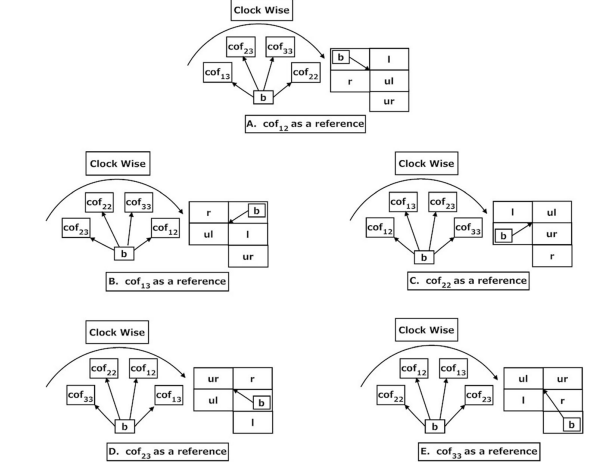
\includegraphics[width=0.6\textwidth]{./img/dct_match_coeff_order.png}
	\caption{\label{fig:coeff_order} Pozycja współczynnika referencyjnego, a wektor wzorca. Źródło:DOI: 10.1007/s11042-017-4676-z}
\end{figure}

Tak ustalony schemat $P$ mapujemy na liczbę postaci:
\begin{equation}
    M(P,S) = P[1]S^3\space + \space P[2]S^2\space + \space P[3]S\space + \space P[4] 
\end{equation}
gdzie $P[i]$ to i-ta współrzędna wektora schematu. W efekcie dla danej pozycji ramki otrzymujemy 2 wartości: $M(P_{max}, S)$ oraz $M(P_{min}, S)$.\\ 

Zliczanie wzorców dla danego obrazu polega na inicjalizacji wektora $T$ o długości $S^4$ (w naszym wypadku 256) zerami. Podczas iteracji ramki po macierzy współczynników dla każdej pozycji wyznaczamy dwie wartości $M_{max}$ oraz $M_{min}$, zgodnie z opisaną metodą, a następnie aktualizujemy wektor $T$: 
\begin{equation}
    T[M_{max}] \mathrel{+}= 1 \space \land \space 
    T[M_{min}] \mathrel{+}= 1
\end{equation}
Kalibracja polega na otrzymaniu wektora cech na podstawie wektorów $T_{org}$ i $T_{crop}$, odpowiednio obrazu oryginalnego i okrojonego. Zauważmy, że różnica w wymiarach tych obrazów nie ma wpływu na wymiary wektorów $T_{org}, T_{crop}$ i oba te wektory są długości $S^4$. Wektor $F$ cech obrazu jest zdefiniowany jako:
\begin{equation}
    F[i] = \frac{T_{org}[i]}{T_{crop}[i]} \space \space i=0,...,S^4-1
\end{equation}
Następnie przeprowadzamy jeszcze normalizację wektora cech:
\begin{equation}
    F[i] = \frac{F[i] - min}{max - min}
\end{equation}
gdzie $min$ i $max$ to odpowiednio najmniejsza i największa wartość wektora cech przed normalizacją. Tak otrzymany wektor cech obrazu przekazujemy do klasyfikatora w celu uczenia bądź klasyfikacji.

\subsection{Klasyfikator oraz Wyniki}
W implementacji użyłem klasyfikatora SVC (Support Vector Classifier), o kernelu Gaussowskim. W celu uzyskania optymalnych parametrów przeprowadziłem przeszukanie (Grid-Search) po siatce:
\begin{equation}
    C \in \{ 2^{-5}, 2^{-4}, ..., 2^{15}\} \space \land \space 
    \gamma \in \{ 2^{-15}, 2^{-14}, ..., 2^3\}
\end{equation}
Zbiór danych (500 obrazów cover i 500 obrazów stego) podzieliłem na zestaw uczący/testowy w proporcji 800/200, z zachowaniem balansu klas (po 400 obrazów stego i cover dla zestawu uczącego i po 100 dla zestawu testowego). Przeszukiwanie siatki parametrów przeprowadzane było przez cross-walidację z parametrem kFold = 5. Na rysunku \ref{fig:dct_match_confusion_matrix} przedstawiono macierz pomyłek dla zestawu testowego.

\begin{figure}[ht!]
	\centering
	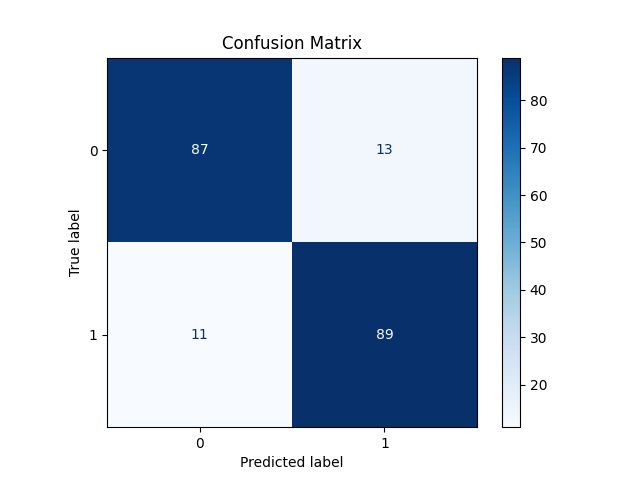
\includegraphics[width=0.7\textwidth]{./img/dct_match_confusion_matrx.png}
	\caption{\label{fig:dct_match_confusion_matrix} Macierz pomyłek dla najlepszego klasyfikatora. Klasa 0 odpowiada obrazom cover, a klasa 1 obrazom stego.}
\end{figure}

Osiągnięto precyzję na poziomię \textbf{88\%}, w tym czułość na poziomie \textbf{89\%} i swoistość \textbf{87\%}.
